\documentclass[a4paper]{article}
\usepackage{amsmath}  % Pacote necessário para \dfrac
\usepackage[utf8]{inputenc}
\usepackage[british,UKenglish,USenglish,english,american]{babel}
\usepackage{graphicx}
\usepackage{array}
\usepackage{fancyhdr}
\usepackage{lastpage} % pacote para obter o número total de páginas
\usepackage{geometry} % pacote para ajustar as margens
\usepackage[datesep=/,style=ddmmyyyy]{datetime2} % pacote para formatar a data
\usepackage{setspace} % Inclui o pacote setspace
\usepackage{enumitem}
\usepackage{amssymb} % Para mais símbolos
\usepackage{indentfirst}
\usepackage{hyperref}
\usepackage{array}
\usepackage{booktabs}

\usepackage{titlesec} % Inclui o pacote titlesec
% Redefinindo o formato do título da seção com um tamanho de fonte menor
\titleformat{\section}
{\normalfont\large\bfseries}{\thesection}{1em}{}

% Definindo margens da página e do cabeçalho
\geometry{
	left=20mm,
	right=20mm,
	top=40mm,
	bottom=30mm,
	headsep=20mm
}

\pagestyle{fancy}
\fancyhf{} % limpa o cabeçalho e rodapé padrão
\renewcommand{\headrulewidth}{0pt} % remove a linha do cabeçalho
\renewcommand{\footrulewidth}{0.4pt} % linha acima do rodapé

\fancyhead[C]{ % conteúdo centralizado no cabeçalho
	\begin{tabular}{|m{3.5cm}|m{9.0cm}|m{3.5cm}|}
		\hline
		\begin{minipage}[c][2.0cm][c]{3.5cm}
			\centering
			
\includegraphics[width=2.98cm,height=1.25cm]{logo.png}
		\end{minipage} & 
		\begin{minipage}[c][2.0cm][c]{9cm}
			\centering
			\hyphenpenalty=10000 % Evita hifenização
			\vspace*{\fill} % Espaço vertical flexível antes do texto
			\begin{spacing}{1.5} % Aumenta o espaçamento entre linhas para 1.25
				{\large \textbf{Inductor for Reducing Transient \textit{Inrush} Current in Capacitors}}
			\end{spacing}
			\vspace*{\fill} % Espaço vertical flexível depois do texto
		\end{minipage} & 
		\begin{minipage}[c][2.0cm][c]{3.5cm}
			\raggedleft
			Issued: \DTMtoday \\
			Page: \thepage/\pageref{LastPage}
		\end{minipage} \\
		\hline
	\end{tabular}
}


% Conteúdo do rodapé
\fancyfoot[L]{%
	\begin{tabular}[b]{@{}l@{}}
		\href{http://www.dax.energy}{www.dax.energy}
	\end{tabular}
}
\fancyfoot[C]{%
	\begin{tabular}[b]{@{}c@{}}
		\href{mailto:comercial@dax.energy}{comercial@dax.energy}
	\end{tabular}
}
\fancyfoot[R]{%
	\begin{tabular}[b]{@{}r@{}}
		+55 41 99940-3744 \\ 3626-2072
	\end{tabular}
}


\begin{document}
	\setstretch{1.25} % Define o espaçamento entre linhas para 1.25
	
	\section{Context}
	The energization of a capacitor bank (Figure \ref{fig:picture1}) by closing a circuit breaker will result in a high transient peak current (Figure \ref{fig:picture2}), called inrush. The magnitude and frequency of this transient peak current are functions of:
	\begin{itemize}[label=\textendash]
		\item the applied voltage (point on the voltage wave at closing);
		\item the equivalent capacitance of the circuit;
		\item the inductance in the circuit (amount and location);
		\item the charge on the capacitor bank at the time of closing;
		\item any damping of the circuit due to closing resistors or other resistance in the circuit.
	\end{itemize}
	
	\section{Input data from the bank}
	\begin{itemize}[label=\textendash]
		\item Reactive power  = {{5.4 MVAr}}
		\item Three-phase voltage  = {{18.0 kV}}
		\item Single-phase voltage  = {{10.4 kV}}
		\item Short-circuit current  = {{2.5 MA}}
	\end{itemize}
	
	\begin{center}
		\begin{tabular}{lllllllllll}
\toprule
 & $Q_{3\phi}$ & $Q_{1\phi}$ & $V_{3\phi}$ & $V_{1\phi}$ & $I_{1\phi}$ & $X_{1\phi}$ & $C_{1\phi}$ & $L_{1\phi}$ & $I_{p}/I_{n}$ & $f_{0}$ \\
\midrule
0 & 1.8 MVAr & 600.0 kVAr & 18.0 kV & 10.4 kV & 57.7 A & 180.0 $\Omega$ & 17.68 µF & 100.0 µH & 97.5 & 3.5 kHz \\
1 & 1.8 MVAr & 600.0 kVAr & 18.0 kV & 10.4 kV & 57.7 A & 180.0 $\Omega$ & 17.68 µF & 100.0 µH & 51.7 & 3.7 kHz \\
2 & 1.8 MVAr & 600.0 kVAr & 18.0 kV & 10.4 kV & 57.7 A & 180.0 $\Omega$ & 17.68 µF & 100.0 µH & 69.0 & 3.7 kHz \\
\bottomrule
\end{tabular}

	\end{center}
	
	
	
	\section{Initial Considerations}
	
	The transient \textit{inrush} current is not a limiting factor in isolated capacitor bank applications. However, when capacitor banks are switched \textit{back-to-back}, i.e., when one bank is switched on while another bank is connected to the same bus, high-magnitude, high-frequency transient currents will flow between the switched bank and those that were already switched on.
	
	\begin{figure}[!hbp]
		\centering
		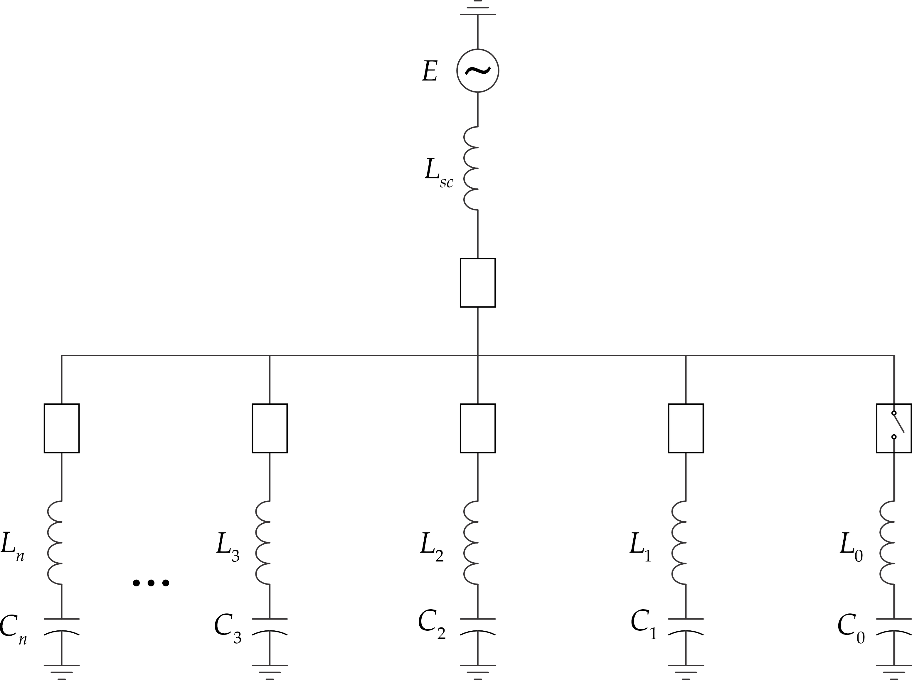
\includegraphics{Picture1.png}
		\caption{Capacitor bank system.}
		\label{fig:picture1}
	\end{figure}
	
	
	This oscillatory current is limited only by the impedance of the capacitor bank and the circuit between the energized bank(s) and the switched bank (Bank \#0), which typically decays to zero within a fraction of a system frequency cycle. In the case of \textit{back-to-back} switching, the component provided by the source is at a lower frequency (60 Hz) and so small compared to the \textit{inrush} current that it can be neglected \href{https://ieeexplore.ieee.org/document/7035261}{[ANSI/IEEE C37.012-1979]}.
	
	\section{Results}
	\begin{figure}[!hbp]
		\centering
		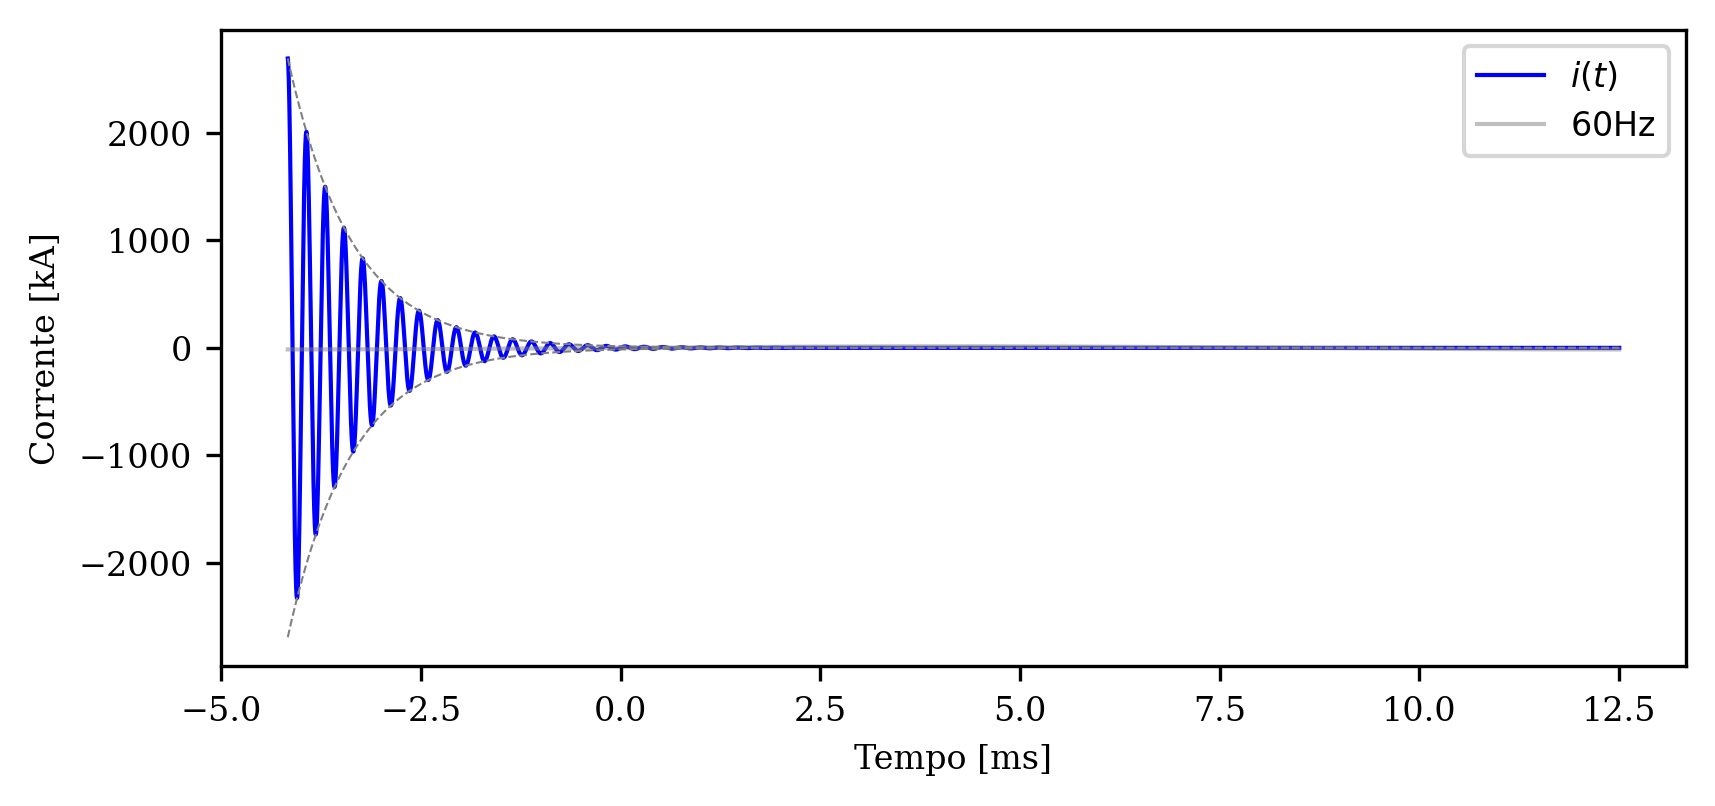
\includegraphics{Correntes.png}
		\caption{Instantaneous current in the capacitor bank switched on in a fundamental frequency cycle.}
		\label{fig:picture2}
	\end{figure}
	
	The values obtained with the selected reactor ($L_{reator} = {{100.0}} \, \mu \rm{H} $) are:
	\begin{itemize}[label=\textendash]
		\item Peak current: {{5.6 kA}};
		\item Oscillation Frequency: {{3.7 k}}Hz;
		\item Inrush current / Nominal current: {{97.5}}
	\end{itemize}
	
	\section{Conclusion}
	{{Adequate reactor, as $\dfrac{I_{\rm inrush}}{I_{\rm nominal}} = $97.47$\le 100$ e $f_{\rm osc} = $3693Hz < 4,25 kHz, IEEE Std C37.012, p. 16[$^{[2]}$](https://ieeexplore.ieee.org/document/7035261) e IEC 62271-100, Table 9 (Preferred values of rated capacitive switching currents), p. 45[$^{[3]}$](https://webstore.iec.ch/publication/62785).}}
	
	\section{References}
	
	\noindent
	\begin{tabular}{p{0.2cm} p{15.8cm}}
		\href{https://ieeexplore.ieee.org/document/7035261}{[1]} &
		\begin{minipage}[t]{15.8cm}
			IEEE Application Guide for Capacitance Current Switching for AC High-Voltage Circuit Breakers Rated on a Symmetrical Current Basis, in ANSI/IEEE C37.012-1979, vol., no., pp.1-54, 6 Feb. 1979, doi: 10.1109/IEEESTD.1979.7035261.
		\end{minipage} \\
		
		\href{https://ieeexplore.ieee.org/document/9574631}{[2]} &
		\begin{minipage}[t]{15.8cm}
			IEEE Approved Draft Standard Requirements for Capacitor Switches for AC Systems (1 kV to 38 kV), in IEEE PC37.66/D10, October 2021, vol., no., pp.1-35, 13 Dec. 2021.
		\end{minipage} \\
		
		
		\href{https://webstore.iec.ch/publication/62785}{[3]} &
		\begin{minipage}[t]{15.8cm}
			IEC 62271-100 High-voltage switchgear and controlgear - Part 100: Alternating-current circuit-breakers
		\end{minipage} \\
		
		\href{https://ieeexplore.ieee.org/document/5318709}{[4]} &
		\begin{minipage}[t]{15.8cm}
			IEEE Standard for AC High-Voltage Circuit Breakers Rated on a Symmetrical Current Basis--Preferred Ratings and Related Required Capabilities for Voltages Above 1000 V, in IEEE Std C37.06-2009, vol., no., pp.1-56, 6 Nov. 2009, doi: 10.1109/IEEESTD.2009.5318709.
		\end{minipage} \\
		
		\href{https://cdn.standards.iteh.ai/samples/101972/4e7e06bd66d2443da668b8e0c6c60512/IEC-62271-100-2021.pdf}{[5]} &
		\begin{minipage}[t]{15.8cm}
			IEC 62271-100 High-voltage switchgear and controlgear – Part 100: Alternating-current circuit-breakers.
		\end{minipage} \\
		
		\href{https://www.normas.com.br/autorizar/visualizacao-nbr/313/identificar/visitante}{[6]} &
		\begin{minipage}[t]{15.8cm}
			NBR 5282 Shunt power capacitors for nominal voltage system above 1000 V.
		\end{minipage} \\
	\end{tabular}
	
	
	
	% Space for signatures
	\noindent % Prevents indentation
	\begin{minipage}[t]{0.5\textwidth} % Starts the first column for signature
		\centering % Aligns text to the center
		\vspace{5cm} % Space reserved for the signature
		\rule{6cm}{0.4pt}\\ % Line for signature
		\textbf{Angelo A. Hafner}\\ % Name
		Electrical Engineer\\ % Title
		CONFEA: 2.500.821.919\\ % Registration number
		CREA/SC: 045.776-5\\ % Another registration number
		aah@dax.energy % Email
	\end{minipage}%
	\hfill % Space between columns
	\begin{minipage}[t]{0.5\textwidth} % Starts the second column for signature
		\centering % Aligns text to the center
		\vspace{5cm} % Space reserved for the signature
		\rule{6cm}{0.4pt}\\ % Line for signature
		\textbf{Tiago Machado}\\ % Name
		Business Manager\\ % Title
		Mobile: +55 41 99940-3744\\ % Contact
		tm@dax.energy % Email
	\end{minipage}
	
\end{document}
